\documentclass[11pt]{article}
\usepackage{a4, fullpage}
\usepackage{bibtopic}
\usepackage[small,compact]{titlesec}
\usepackage{float}
\usepackage{amssymb,amsmath}
\usepackage[T1]{fontenc}
\usepackage{graphicx}
%\usepackage{multicol}
%\usepackage{multirow}
%\usepackage{listings}
%\usepackage{pdfpages}
%\usepackage{booktabs}

%\restylefloat{table}

%\setlength{\parskip}{0.3cm}
%\setlength{\parindent}{0cm}
%\setlength{\textheight}{10.7in} %used to be 10
%\setlength{\textwidth}{6.5in}
%\setlength{\parskip}{2pt}
%\addtolength{\oddsidemargin}{-.3in}
%\addtolength{\evensidemargin}{-.3in}
%\addtolength{\topmargin}{-.6in}
%\addtolength{\textwidth}{.6in}


\begin{document}

%-------------------------------------------------------------------------------

%\title{\vspace{100px} BUSINESS PLAN \\ \vspace{100px} Shimla Gold Cider \vspace{100px}}
%\author{\vspace{50px}John Walker, Rutwik Shah, Sahil Jain, Alina Boghiu, Giovanni Charles, Łukasz Koprowski \vspace{50px}}

%Imperial College London, Department of Computing

%\date{\today}         % inserts today's date

%\maketitle           % generates the title from the data above

%\newpage

%\title{ \hspace{100px} SHIMLA GOLD CIDER BUSINESS PLAN}
%\maketitle

%\begin{table}[H]
%\begin{center}
%\begin{tabular}{| l | l |}
%\hline
%Date Stamp of this Document:     &  \today  \\ \hline
%Version of this Document:        &  V.0.2   \\ \hline
%Author/Editor of this Document:  & Adam Fiksen, \newline Alina Boghiu, \newline Giovanni Charles, \newline John Walker, \newline Rutwik %Shah, \newline Sahil Jain, \newline Lukaz Koprowski  \\
%\hline
%\end{tabular}
%\end{center}
%\end{table}


%-------------------------------------------------------------------------------

%-------------------------------------------------------------------------------
%    ALTERNATIVE TITLE PAGE
%-------------------------------------------------------------------------------

\begin{titlepage}
\newcommand{\HRule}{\rule{\linewidth}{0.5mm}}
\center
\textsc{\LARGE Imperial College London}  \\[1.5cm]
\textsc{\Large Department of Computing}  \\[0.5cm]
\textsc{\large Course 350: Management and Business for Computing Engineers} \\[0.5cm]

\HRule \\[0.3cm]
{\huge \bfseries Business Plan \\ \vspace{0.3cm}Shimla Gold Cider} \\[0.3cm]
\HRule \\[1.5cm]

\begin{minipage}{0.4\textwidth}

% author
\begin{flushleft} \large \emph{Authors:} \\
Alina     \textsc{Boghiu}    \\
Giovanni  \textsc{Charles}   \\
Adam      \textsc{Fiksen}    \\
Sahil     \textsc{Jain}      \\
\L ukasz  \textsc{Koprowski} \\
Rutwik    \textsc{Shah}      \\
John      \textsc{Walker}    \\
\end{flushleft}

% supervisors
\end{minipage}~
\begin{minipage}{0.4\textwidth}

\begin{flushright} \large \emph{Lecturer:} \\
Nick \textsc{Coutts}
\end{flushright}
\end{minipage}\\[4cm]

%
\includegraphics[width=\textwidth]{apples.jpg}
\end{titlepage}

%-------------------------------------------------------------------------------
\title{DISCLAIMER}
\maketitle

\noindent This business plan has been prepared by the authors and is being provided to a limited number of persons, at their request. This document is confidential and is only being made available to parties who agree to keep it confidential. Neither this business plan nor any part of it shall be copied, reproduced or distributed to others at any time without the prior written consent of the authors. By accepting this document the recipient is deemed to undertake and warrant to the authors that the recipient will keep it confidential and that the recipient shall return all copies of this document to the authors immediately upon request. \\

\noindent Although X has taken reasonable care to ensure that the information contained in this document is accurate, no other representation or warranty, express or implied, is or will be given by X or any of its agents. No responsibility is or will be accepted by the authors or any of its agents as to the accuracy or completeness of this document or the information or opinions contained herein. Recipients must make their own investigations and must satisfy themselves as to the condition and prospects of the authors and the accuracy and completeness of statements contained herein. \\

\noindent Any financial projections given in this plan are illustrative only. Because of the early stage nature of the authors’ business, none of the projections given in this document should be taken as guaranteed to be attainable, nor should they be taken as implying any indication, assurance or guarantee that those assumptions are correct or exhaustive.
\vfill
\begin{table}[H]
\begin{center}
\begin{tabular}{| l l |}
\hline
Issued To:      &  Nick Coutts        \\
Company:        &  Shimla Gold Cider  \\
Date of Issue:  &  \today             \\
Copy Number:    &  1                  \\
\hline
\end{tabular}
\end{center}
\end{table}

\newpage
\tableofcontents
\newpage

%------------------------EXECUTIVE SUMMARY-------------------------------------%
\section{Executive Summary}
  \subsection{Overview}

  %A patented solution...
  %Vision to be...
Our mission is to bring a mid priced cider to the people of India. India has the second largest population in the world, and has an estimated market size of 500 million alcohol consumers [better estimate]. At the moment, there is one provider of cider in India, and we would like the change that. \\

\noindent We want to be a brewery. We will brew our own cider in the state of Himachal Pradesh, which is the source of the majority of the apples in India. Along with producing cider, we will sponsor other exclusive bars and clubs. \\

\noindent Operating in India which is well known for its corruption, we want to practice ethical development. eg corrupt free, no bribes, no blood cider forced labour fairtrade \\

\noindent We hope to gain popularity in major establishments, in Delhi and Mumbai through the open minded youth and bar owners. \\

\noindent Our cider will become a desired commodity through exclusivity and we will be able to research our market further at this point with minimal risk. \\

\noindent We will adapt and pick up popularity and scale up to make it available to the public.
  %Consumer and regulatory pressure...
  %Has clear competitve advantages...
  %Has unsurpassed technology and has sales through...

  \subsection{Market Drivers}
  %Market drivers....
\noindent Our proposed route to market begins with the launch of a microbrewery in [city]. \\

\noindent [Explaination of our brewpub] \\

  \subsection{Business Proposition}
  %Meets increasing demands...
  \subsection{Financial Summary and Investment Proposition}
  %Requires...


%------------------------------------------------------------------------------%
%------------------------MARKET OPPORTUNITY------------------------------------%
\section{Market Opportunity}

\subsection{Market Analysis}
  \subsubsection{Current Competitors in the Cider Market}
At the moment, there is only one company which produces cider in India. The company, Green Valley Cider, produces Tempest Cider in the state of Himachal Pradesh, where they own several acres of apple orchards.

  \subsubsection{Current Competitors in the Microbrewery Market}
  \begin{itemize}
  \item Rockman's Beer Island, Gurgaon - Located in the largest shopping mall in Gurgaon (bordering New Delhi), Rockman's Beer Island was India's first micro pub brewery. They offer four types of beer: Lager Strong Beer, Dark Beer, Lager Beer and Wheat Beer, and they aim to serve some exclusive flavoured beers by the summer. Along with the micro pub brewery, they also own an exclusive German restaurant and a digital auditorium covering an area of around 3500 m$^2$. Rockman's are planning to expand now by opening their branch in different locations in India.
  \item Toit, Bangalore - Located in the Technology capital of India, Toit has been doing really well since it has opened. They offer 6 different types of beers, which are Toit's Basmati Blonde, Tintin Toit, Toit Weiss, Toit Red, Colonial Toit and Toit's Dark Knight. They are currently in the process of introducing exclusive Toit merchandise, along with their wide selection of food and alcohol. Toit are planning on making the branch national by the end of this year.
  \item The Biere Club, Bangalore - Another micro pub brewery which is located in Bangalore, The Biere Club also brews around 6 different types of beers, which include Lager, Ale and Wheat. The Biere Club are planning on making partnerships with rich individuals for expansion in the future.
  \item Doolally, Pune - Located in Pune, Doolally has been operational for around three years. It is located in a boutique hotel, and plans to open in a few more locations soon.
  \end{itemize}

  \subsection{The Opportunity for Shimla Gold Cider}
As we can see, there is a large market for alcohol in India, who are eager to try out new things, which can be seen by the successes of these microbreweries. As India continues to grow to become a bigger powerhouse in the world, it will attract more foreigners, which means that people who already know about cider and like it will increase in the country. This increasing market size makes us believe that cider will become increasingly popular in India once introduced properly.
  %Addressable market of... 
 
  \subsection{Market Segments}
  %Clear market segments Including...


%------------------------------------------------------------------------------%
%------------------------PRODUCT PROPOSITION-----------------------------------%
\section{Shimla Gold Cider Product Proposition}
%Has superior technology in....
  \subsection{Shimla Gold Cider's Unique Proposition}
  %Is proven cost effective and easy to implement...
  \subsection{Business Model}
  \newpage
  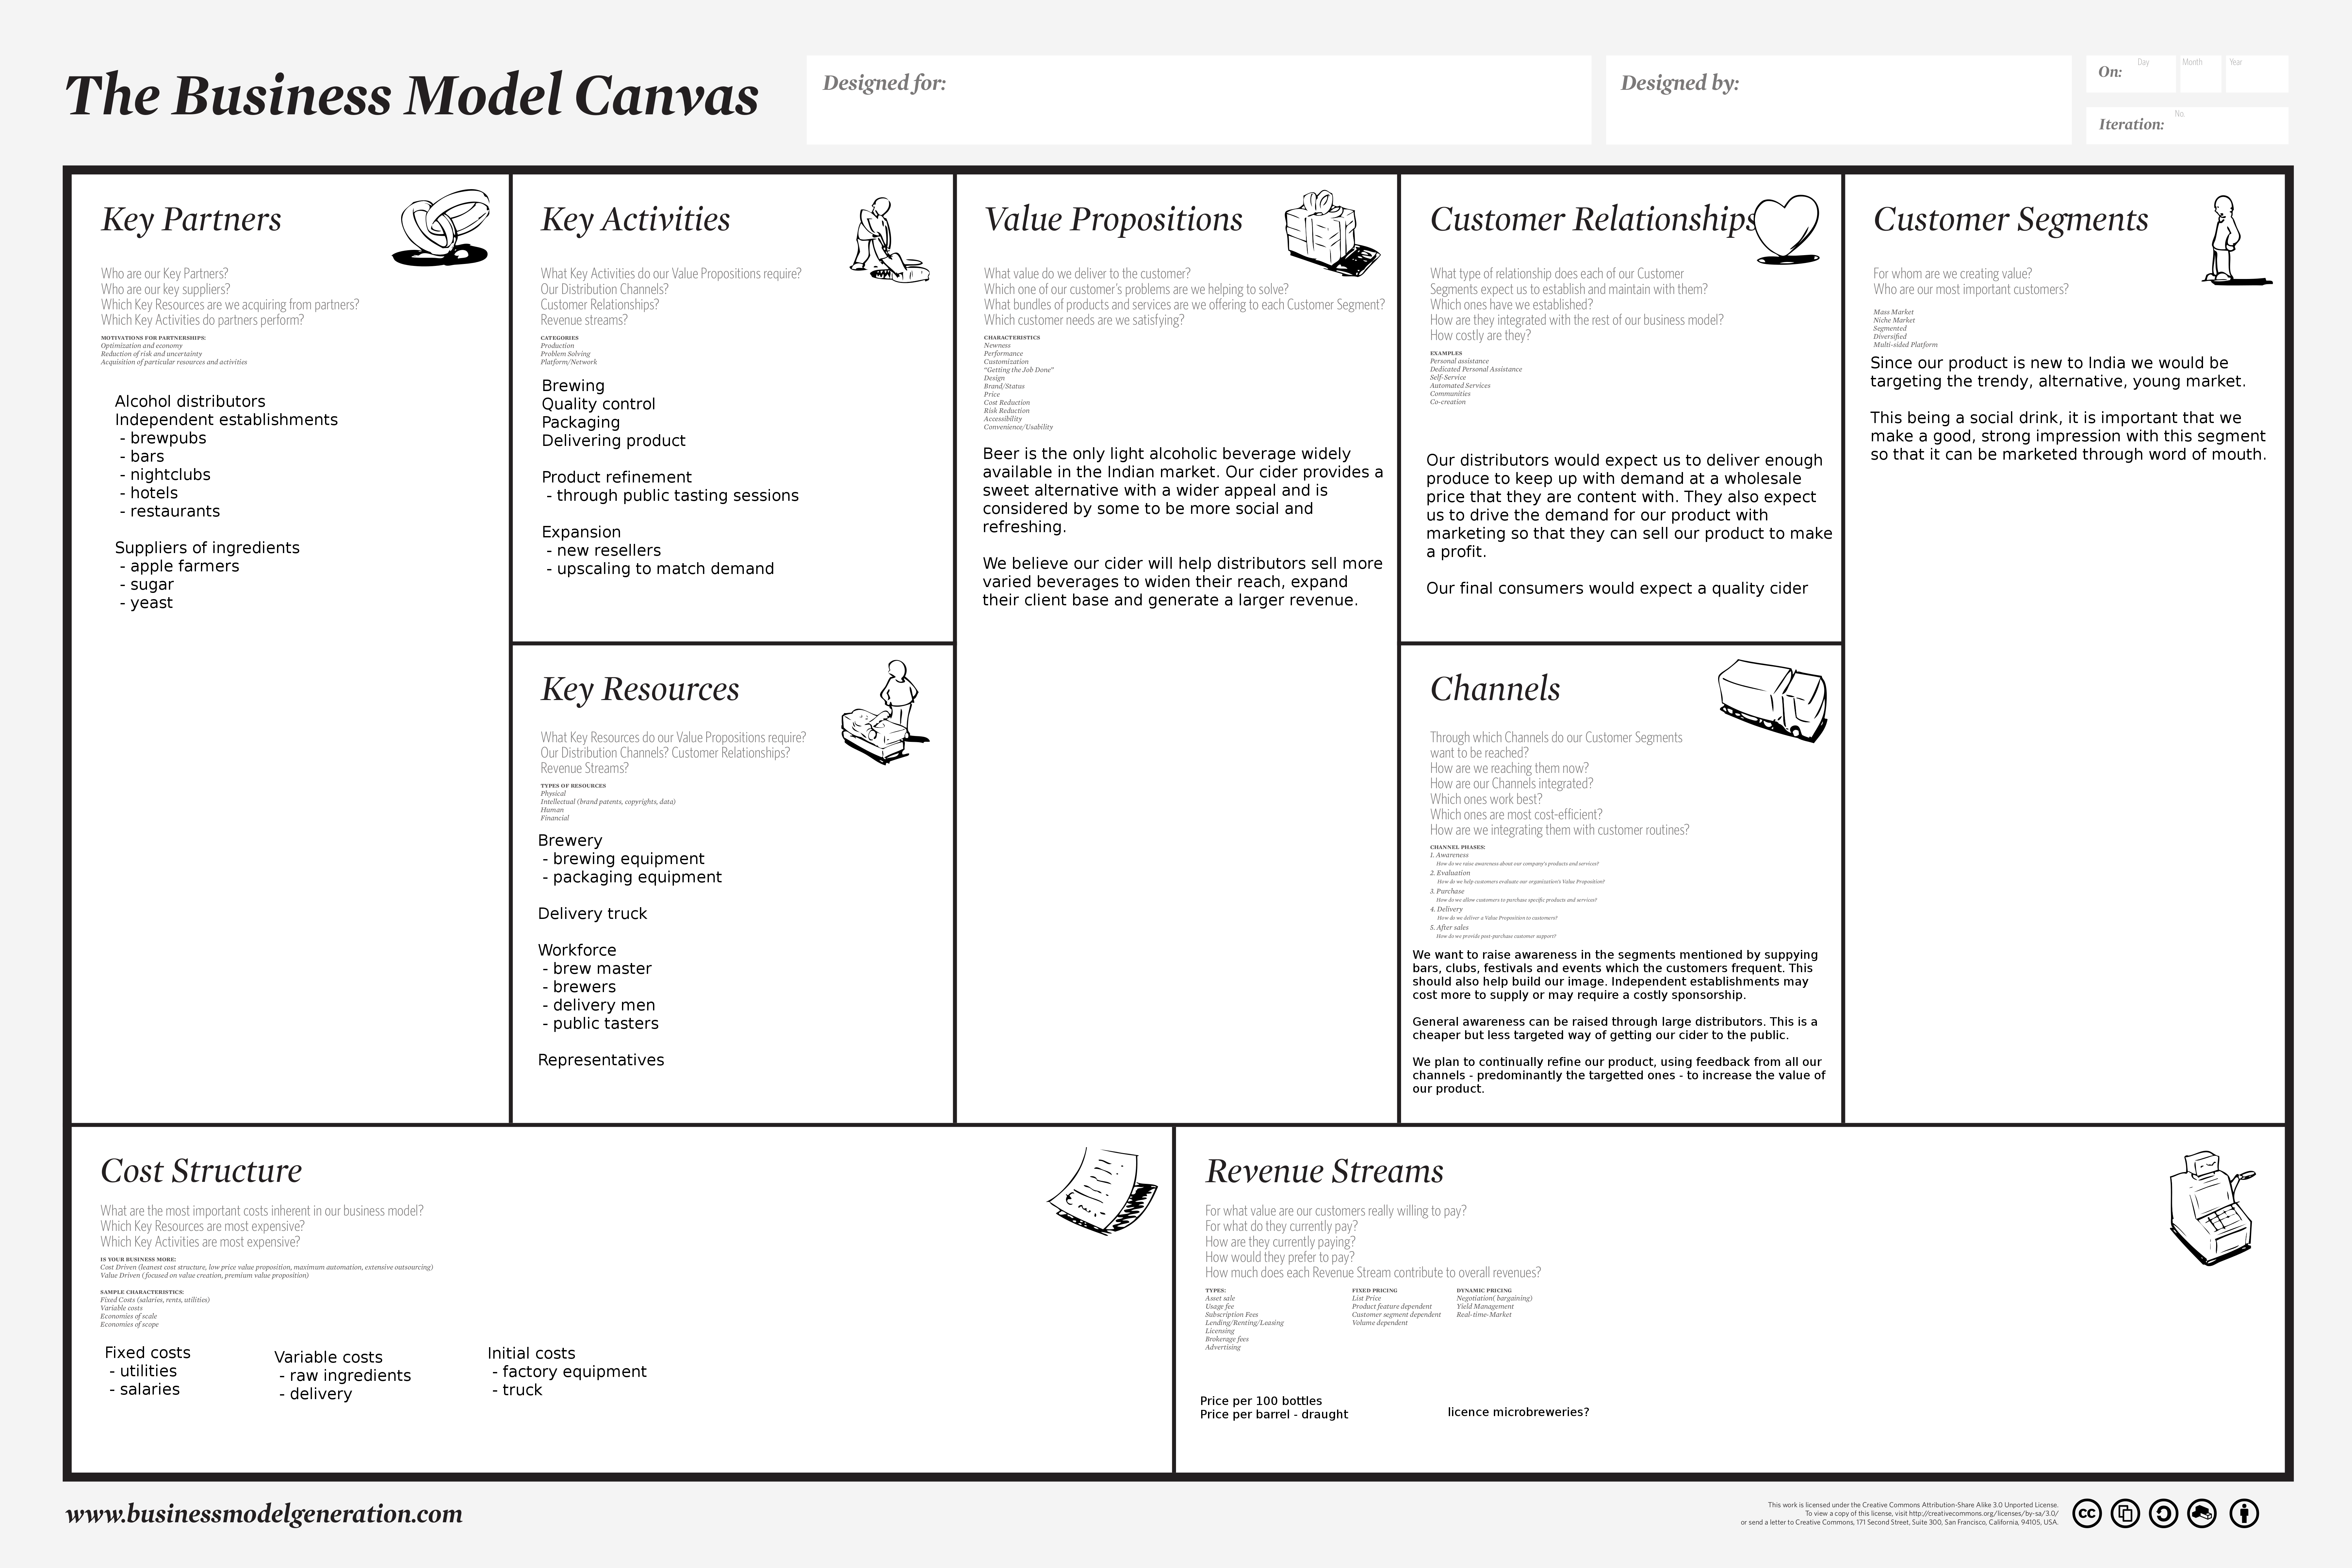
\includegraphics[angle=90,width=\textwidth,height=\textheight,keepaspectratio]{./business_model_canvas_poster.png}
   %Established production, sales & marketing, distibution model...


%------------------------------------------------------------------------------%
%------------------------TARGET MARKET-----------------------------------------%
\section{Target Market}
  \subsection{Market Context}
  %Global vision well defined market segments and territories...
  \subsection{Market Size and Characteristics}
  %This equates to a global revenue opportunity of??? 
  %Diagram yearly market potential
  \subsection{Market Validation}
  %Has met all technical norms


%------------------------------------------------------------------------------%
%------------------------MARKET DEVELOPMENT PLAN-------------------------------%
\section{Market Development Plan}
  \subsection{Sales Process}
  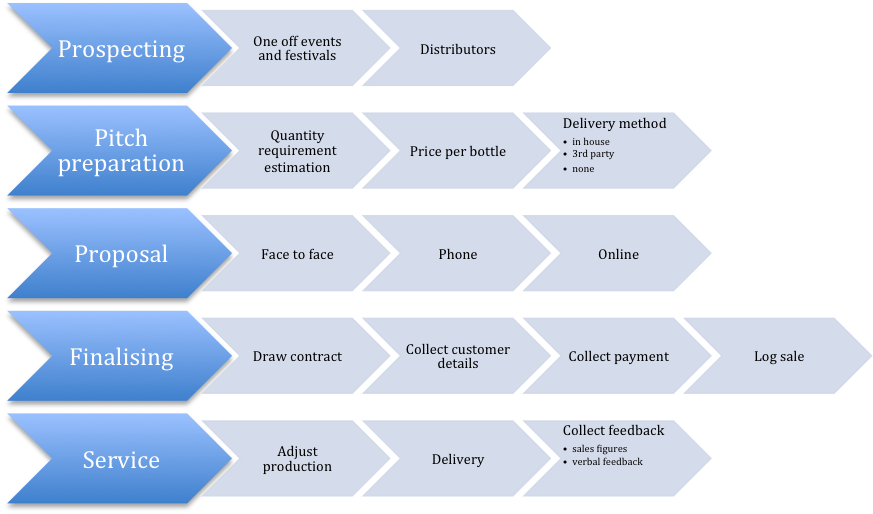
\includegraphics[width=\textwidth,keepaspectratio]{./process.png}
  %Proven sales process...
  %Good relationship with strong distributor...
  %\subsection{Target Customers}
  %Larger customers as targets
  %\subsection{Current Key Customers}
  %Large current customers
  \subsection{Marketing, PR and Communications}
We aim at advertising at horse racing events this has a cost of Rs. 5,00,000 though this number is high it has several benefits in doing so:
\begin{enumerate}
\item Conduct contests of skill and award prizes to the public to generate interest. 
\item Advertise on the CCTV transmission at all centers .
\item Have full rights for on-site branding across the stands.
\item Name the race to suit its preference.
\item Have its CEO / nominee present the trophy.
\item Be entitled to the free use of lawns above a certain value of sponsorship.
\item Arrange for live entertainment at race time or before or after the event.
\item Promote and your brand the race via mailers/press.
\item Have access to the Club's membership data which consists of thousands of potential customers who represent some of the most well off clients in India.
\item Have promotion on the website with links to the lounges webpage.
\item Get coverage on a major television network as these races will be viewed world wide.
\end{enumerate}


%------------------------------------------------------------------------------%
%------------------------COMPETITION-------------------------------------------%
\section{Competition}
%Limited number of direct competitors
  \subsection{Competitive Advantage}
  %Competitve advantage in technology


%------------------------------------------------------------------------------%
%------------------------INTELLECTUAL PROPERTY (IP) ASSETS---------------------%
\section{Intellectual Property (IP) Assets}
  \subsection{Shimla Gold Cider Solution}
    \subsubsection{Patents}
    %Technology protected 1. 2. 3. ....
    \subsubsection{Know-How}
    %Internation experts choose to work with X
  \subsection{Future IP Developments}
  %Future applications plannes along with IP Protection...


%------------------------------------------------------------------------------%
%------------------------BUSINESS GROWTH AND RESOURCE PLANS--------------------%
\section{Business Growth and Resource Plans}
In order to setup a stable and longlasting infrastructure for our business we must take into consideration all the stages and requirements of production. Reaserching our cider recipe constituted the guideline and starting point of a coherent development plan. 

  \subsection{Current Structure and Resources}
  %Early phase centred on technology development
When deciding upon our homebase structure we considered firstly our situation as a new business, with no existing assets or experience, as well as a reasonable aim of setting up a small scale production line.

The favourable aspects of our current situation is our team of young, dynamic individuals, excited about implementig a good business idea. We are fast learners, on our way to obtaining university degrees, with a great tolerance to change and fully capabale of taking on unforseen obstacles without being overwhelmed by minor defeats. We believe a positive, persistent and energetic attitude towards implementig any business will yield a positive result and a great learning experience.

  \subsection{Straff Recruitment}
%The average cost of hiring for the skilled workers is about 1,00,000 a year we would require :

% Keep all the cost and finance information in one well defined section

  \begin{enumerate}
  \item Qualified Brewmaster \\
He has to have previous experience with brewing various types of cider and would probably have to be recruited from a country with cider making traditions (France, England). He would serve as our cider making expert, being able to swiftly operate the equipment and professionally asses the quality of our cider. He must also supervise the general staff activity and behaviour.

  \item Microbiologist \\
He would serve as an assistant brewmaster, and would be responsible for conducting cider quality control tests, and performing microbiological analysis. He must also verify all the ingredients including the apples, sugar, yeast and water.
It is important to ensure a good quality especially considering the novelty of our product for this market.

  \item Unqualified labour \\
Our microbrewary requires manual labour as described below. These employees must work with the equipment we provide, attend to washing and maintaing it with resposability. Therefore brief training must be considered as a cost. \\ 
  2 workers in charge of apple receival, washing and sorting
  2 workers in charge of apple grating
  2 workers in charge of apple pressing
  1 worker in charge of general cleaning of the area

  \item Security guard \\
On top of general surveillence, he is in charge of verifying employee ids and greeting visitors.
  \end{enumerate}

% same here, all cost information in one place

% Further as required we will require a security guard which will cost about Rs. 50,000 a year.
 
  \subsection{Facilities}
    \subsubsection{Space requirements}
When deciding upon our homebase we considered firstly our situation as a new business, with no existing assets or experience, as well as the small scale of our production line. \\

We are aiming to brew \emph{15 gallons per day}. Whilst we will start off by brewing small qunatities in order to perfect the recipe, we must setup the scale which we need for efficient and profitable distribution. We have already identified the ingredients qunatity requirements per gallon when researching the recipies we will use and have explained how these might change. Using this information, these are the room size and functionality requirements we identified: \\

  \begin{enumerate}
  \item Ingredients handling room \\
  This room must be easily accessible by our providers and large enough to store a week's worth of ingredients including: \\
    \begin{itemize}
    \item 1500L refrigerator to store 630Kg of apples
    \item 23kg of sugar
    \item yeast, campden tablets
    \end{itemize}
  The room must have a constant supply of water for washing apples and equipment. \\
  The room will operate a weekly pipeline of ingredients storage, however spare space must be available for unforseen situations.\\
  The room size must also allow washing, grating and pressing of apples which implies equipment and staff as detailed in the following sections.

  \item Brewing room \\
  This room must accomodate the two brewing systems for dry and sweet cider: aproximately $2m^3$ each. It must also be able to fit a desk and file cabinet for general office equipment.
  \item Fermenting room \\
  This room will operate a daily pipeline and must be able to accomodate a weeks worth of produce: $4m^3$. It must maintain a constant temperature of aproximately $22^\circ$C for fermentation. We have decided upon this as a good trade-off between quality and speed which are inveresely proportional: a lower fermenting temperature yelds higher quality but requires more time. However this is a specific decision the brewing master must make daily.

  \item Bottling and storage room \\
  This room must accomodate
% Adam, a pargraph here please

  \item Maintainance room\\
  This should be a small room for storing cleaning equipment. It should have access or be attached to a staff restroom.
  \end{enumerate}

    \subsubsection{Equipment requirements}
    \begin{enumerate}
    \item Production equipment
      \begin{itemize}
      \item Apple wash tub
      \item Apple crushing device
      \item Hand cracked cider press: small
      \item Mash tank: 15 gallon
      \item Sparge tank: 15 gallon
      \item Boil Kettle with a false bottom and a siphoning tube
      \item Chill wizzard with a cold water hoze and oxigen pump
      \item Fermenting tank with blow up valves for speedup: 15 gallon
      \item Propane burner
      \end{itemize}

    \item Storage equipment
      \begin{itemize}
      \item 1500L refridgerator for apple storage
      \item freezer for excess and spare apple woat
      \item Fermenting tanks: as mentioned above, in order to host the weekly pipeline, we require 7 15 gallon tanks and spares.
      \item bottles: we are aiming for a production line of 210 bottles daily therefore our weekly requirements is of aproximately 1300 bottles including spares
      \item boxes and lables
      \item shelves or containers ingredients (which come in their own boxes)
      \end{itemize}

    \item General maintainance equipment
      \begin{itemize}
      \item airconditioning system: for the fermentation process
      \item security alarm ans surveillence system
      \item fire detection system
      \item water filtering system
      \item cleaning equipment: \\
        \begin{itemize}
        \item chemical substances (pbw socution, idophor)
        \item cleaning substances (soap, bleach)
        \item blue roll, toilet roll, cloths
        \item bags, bin bags
        \item hozes, gloves, brooms, mops, buckets
        \end{itemize}
      \item office equipment:
        \begin{itemize}
        \item paper and pens
        \item company stamp, files, plastic sleeves, paper punch, envelopes, stapler and spaples, disposable cups, bin
        \item employee register book, visitor register book
        \item company landline telephone
        \item company laptop
        \item tea, coffee, water
        \item first aid kit
        \end{itemize}
      \end{itemize}
    \end{enumerate}

%------------------------------------------------------------------------------%
%------------------------FINANCIAL PLAN AND FUNDING ASSUMPTIONS----------------%
\section{Financial Plan and Funding Assumptions}
  \subsection{Financial History}
  \subsection{Financial Projections}
Initially our main source of revenue would stem from sale of products in the short run once we aim at establishing our brand through adverstising and selling through pubs. Gradually we would like to further increase volume of sales and production and increase revenue through sponsors. In the long run we would like to further increase our product range including different flavours of ciders and gradually streamline our distribution process. This will all result in economies of scale hence reducing cost and added prodict range will increase volume of sales.

  \subsection{Use of Funds}
      \subsubsection{Staff Hiring and Property}
Since we aim at setting up a microbrewery to start with in at a manufacturing area in Himachal Pradesh

Rent in this area is roughly about Rs.1 / ft$^2$ per month.
As seen in the requirements:

there is a storage area required this has been estimated to: 500 sq $^2$ area of for manufacturing the product would be 1500 ft$^2$ this is plenty to space to meet estimated current requirements

Lunch area and office space is estimated to be about 1000 $^2$ as well this as above well allows some space for hiring a few more employees if and when needed.

Hence yearly rent works out at Rs. 24,000 per year.
   \subsubsection{Ingredients}
cost of sugar -  Rs.30 / kg
campden tables  - Rs.300 per 100 tablets
Sweet mead Rs.500 for /128 gms 


This brings the cost of dry cider to Rs. 5.866 per 330 ml
This brings the sweet of dry cider to Rs. 6.4 per 330 ml

\subsubsection{Equipment and Facilities}
  %Funds needed for sales and marketing support


%------------------------------------------------------------------------------%
%------------------------EXIT STRATEGY-----------------------------------------%
\section{Exit Strategy}
%Exit-trade sale


%------------------------------------------------------------------------------%
%------------------------RISK ANALYSIS-----------------------------------------%
\section{Risk Analysis}

  \subsection{Risk Assessment and Management}
  Identyfying risks is mainly aimed at helping to outline a realistic budget requirement. Most of the items below are not avoidable, like staff illness or natural hazzards. However some are, and foreseeing even the unavoidable ones can make them more managable. Following is a comprehensive list of risks, including our approach to dealing with them.
   %Strong distribution channels minimise risk as does IP protection

  \begin{enumerate}
  \item human related
    \begin{itemize}
    \item Delaied production \\ Wheather it is because of suppliers delivering ingredients late or to do with the quality of the delivered product, we should have either a week's worth safety batch, which implies buying a freezer, or be prepared to deal with the cost of delaied production. \\

    \item Late distribution \\
The small scale of our buiness means space is limited which may cause a problem if buyers are late with picking up the merchandise. We should consider having an emergenci courier  or again be prepared to deal with the const of delaied production.
    \item Experience of employees \\
Providing a training session is sometimes insufficient for ensuring perfect performance from our employees. We must be prepared to deal with the cost of flawed batches.
    \item injuries, illness \\

 (spare trained professional), misbehaviour
    \item security (24h, think key priveleges: already existent)
    \item working conditions: 
    \end{itemize}

  \item equipment related risks
    \begin{itemize}
    \item breaks (replacements) (have backup?)
    \item power cuts (generator backup? - some need: fridge etc.)
    \item water contamination 
    \item moldy apples
    \item run out of storage space (redundant storage)
    \end{itemize}

  \item ethical risks
    \begin{itemize}
    \item working environment
    \item religious employees
    \item local water supply, disposal of waste (donate apple waste)
    \end{itemize}
  \end{enumerate}
%------------------------------------------------------------------------------%
%------------------------COMPANY STRUCTURE AND MANAGEMENT PROFILES-------------%
\section{Company Structure and Management Profiles}
  \subsection{Current Equity Structure}
  %Clear ownership structure
  \subsection{Management Team}
  %Expirences management team
  \subsection{Corporate Information}
  %Directors
  %Registered Number
  %Registered Office
  %VAT Number
  %Company Auditors
  %Company Lawyers
  %Company Bankers
  \subsection{Location and Contact Details}


%------------------------------------------------------------------------------%
%------------------------MARKET PLAYERS----------------------------------------%
\section{Market Players}


%------------------------------------------------------------------------------%
%------------------------ANNEX 1-----------------------------------------------%
\section{ANNEX 1}

%this is not an annex but a conclusion sumerising our learning outcomes
As a conclusion to our business proposition we would like to outline a few learning outcomes this experience has provided us with.\\

Fisrtly, being put in the situation of having to think about the implementation details of a business has shown us the benefits of being able to follow a well defined plan and the advantages of being organized as a team. Whilst the business idea might be fairly easy to explain, its implementation, however small the scale, raises an edless stream of problems to be solved and questiones to be answered which prove both the capacity and the limitations of human intuition. For this reason it is extreamly important to follow a rigurous plan and try to forsee as many risks as possible, as it is impossible to control the flow of events completely. \\

Secondly, we learnt there is much more to selling a product than making it available. Whilst a good product will advertise itself, tiit is important to sell the entire experience that goes with it and be prepared for both expantion or having to start over from scratch. Looking at success and failiure stories of other startups whilst trying to outline the plan for our own business developement, we saw that luck, whilst helpful, is replaceable with careful financial estimations, a pesimistic timeline and clever safety measures. \\

Finally, we saw that in order to make good use of resources and come accross as reliable the leading team must have well defined roles, in accordance with their skills. in order for potential investors to trust we can acomplish our goals, it is important to have a constant sense check when planning developement and remain realistic.\\

We consider this exercise to have been a worthwhile experience for having shown us a more comprehensive way of thinking about projects in general.


%------------------------------------------------------------------------------%
%------------------------ANNEX 2-----------------------------------------------%
\section{ANNEX 2}


%------------------------------------------------------------------------------%
%------------------------ANNEX 3-----------------------------------------------%
\section{ANNEX 3}


%------------------------------------------------------------------------------%
%------------------------COMPANY BACKGROUND------------------------------------%
\section{Company Background}


%------------------------------------------------------------------------------%
\end{document}
